\documentclass{beamer}
\usepackage[utf8]{inputenc}
\usetheme{Madrid}
\usecolortheme{default}
\usepackage{amsmath,amssymb,amsfonts,amsthm}
\usepackage{txfonts}
\usepackage{tkz-euclide}
\usepackage{listings}
\usepackage{adjustbox}
\usepackage{array}
\usepackage{tabularx}
\usepackage{gvv}
\usepackage{lmodern}
\usepackage{circuitikz}
\usepackage{tikz}
\usepackage{graphicx}
\setbeamertemplate{page number in head/foot}[totalframenumber]
\usepackage{tcolorbox}
\tcbuselibrary{minted,breakable,xparse,skins}
\definecolor{bg}{gray}{0.95}
\DeclareTCBListing{mintedbox}{O{}m!O{}}{%
breakable=true,
listing engine=minted,
listing only,
minted language=#2,
minted style=default,
minted options={%
linenos,
gobble=0,
breaklines=true,
breakafter=,,
fontsize=\small,
numbersep=8pt,
#1},
boxsep=0pt,
left skip=0pt,
right skip=0pt,
left=25pt,
right=0pt,
top=3pt,
bottom=3pt,
arc=5pt,
leftrule=0pt,
rightrule=0pt,
bottomrule=2pt,
toprule=2pt,
colback=bg,
colframe=orange!70,
enhanced,
overlay={%
\begin{tcbclipinterior}
\fill[orange!20!white] (frame.south west) rectangle ([xshift=20pt]frame.north west);
\end{tcbclipinterior}},
#3,
}
\lstset{
language=C,
basicstyle=\ttfamily\small,
keywordstyle=\color{blue},
stringstyle=\color{orange},
commentstyle=\color{green!60!black},
numbers=left,
numberstyle=\tiny\color{gray},
breaklines=true,
showstringspaces=false,
}
\title
{4.11.20}
\date{September 29, 2025}
\author
{EE25BTECH11043-Nishid Khandagre}
\begin{document}
\frame{\titlepage}
\begin{frame}{Question}
Find the coordinates of the point where the line through the points $\vec{A} \myvec{3\\4\\1}$ and $\vec{B}\myvec{5\\1\\6}$ crosses the $XZ$ plane. Also find the angle which this line makes with the $XZ$ plane.
\end{frame}
\begin{frame}{Theoretical Solution}
Direction vector
\begin{align}
\vec{d} &= \vec{B} - \vec{A}\\
&=\myvec{5 \\ 1 \\ 6} - \myvec{3 \\ 4 \\ 1} = \myvec{2 \\ -3 \\ 5}
\end{align}
The normal vector $\vec{n}$ to the $XZ$-plane is:
\begin{align}
\vec{n} = \myvec{0 \\ 1 \\ 0}
\end{align}
\end{frame}
\begin{frame}{Theoretical Solution}
General point $\vec{P}$ on the line:
\begin{align}
\vec{P} = \vec{A} + t\vec{d}
\end{align}
For the line to intersect the $XZ$-plane, the point $\vec{P}$ must lie on the plane.
Therefore
\begin{align}
\vec{n}^\top\vec{P}&=0\\
\vec{n}^\top(\vec{A} + t\vec{d}) &= 0 \\
\vec{n}^\top \vec{A} + t (\vec{n}^\top \vec{d}) &= 0 \\
t &= -\frac{\vec{n}^\top \vec{A}}{\vec{n}^\top \vec{d}}
\end{align}
\end{frame}
\begin{frame}{Theoretical Solution}
\begin{align}
\vec{n}^\top \vec{A} &= \myvec{0 & 1 & 0} \myvec{3 \\ 4 \\ 1} =4 \\
\vec{n}^\top \vec{d} &= \myvec{0 & 1 & 0} \myvec{2 \\ -3 \\ 5}= -3
\end{align}

\begin{align}
t = -\frac{4}{-3} = \frac{4}{3}
\end{align}
\end{frame}
\begin{frame}{Theoretical Solution}

Intersection Point
\begin{align}
\vec{P} &= \vec{A} + \frac{4}{3}\vec{d}\\
&=\myvec{3 \\ 4 \\ 1} + \frac{4}{3}\myvec{2 \\ -3 \\ 5}\\
& = \myvec{\frac{17}{3} \\ 0 \\ \frac{23}{3}}
\end{align}

\end{frame}
\begin{frame}{Theoretical Solution}
The angle $\theta$ between a line with direction vector $\vec{d}$ and a plane with normal vector $\vec{n}$ is given by:
\begin{align}
\sin\theta = \frac{|\vec{n}^\top \vec{d}|}{\norm{\vec{n}}\norm{\vec{d}}}
\end{align}
\begin{align}
\norm{\vec{n}}=\sqrt{\vec{n}^\top\vec{n}}
\end{align}
\begin{align}
\norm{\vec{n}}&=\sqrt{0^2 + 1^2 + 0^2}\\
\norm{\vec{n}}&= 1
\end{align}
\begin{align}
\norm{\vec{d}}=\sqrt{\vec{d}^\top\vec{d}}
\end{align}
\begin{align}
\norm{\vec{d}}&= \sqrt{2^2 + (-3)^2 + 5^2}\\
\norm{\vec{d}}&=\sqrt{38}
\end{align}
\end{frame}
\begin{frame}{Theoretical Solution}
\begin{align}
    \sin\theta &= \frac{|-3|}{1 \cdot \sqrt{38}} = \frac{3}{\sqrt{38}}
\end{align}
\end{frame}

\begin{frame}[fragile]
\frametitle{C Code}
\begin{lstlisting}
#include <math.h> 

// Function to calculate the intersection point and angle
void findIntersectionAndAngle(
double x1, double y1, double z1,
double x2, double y2, double z2,
double *ix, double *iy, double *iz,
double *angle_degrees) {

// Direction vector of the line (L = B - A)
double Lx = x2 - x1;
double Ly = y2 - y1;
double Lz = z2 - z1;
\end{lstlisting}
\end{frame}
\begin{frame}[fragile]
\frametitle{C Code}
\begin{lstlisting}
// Parametric equation: P(t) = A + t * L
// P(t) = (x1 + t*Lx, y1 + t*Ly, z1 + t*Lz)
// For the XZ plane, y-coordinate must be 0:
// y1 + t*Ly = 0  => t = -y1 / Ly
double t = -y1 / Ly;
// Calculate the intersection point coordinates
*ix = x1 + t * Lx;
*iy = y1 + t * Ly; // Should be 0
*iz = z1 + t * Lz;
// Calculate angle with XZ plane (normal N = (0,1,0))
// sin(theta) = |L . N| / (||L|| * ||N||)
// L . N = Ly, ||N|| = 1
double dot_product = Ly;
double magnitude_L = sqrt(Lx * Lx + Ly * Ly + Lz * Lz);
double sin_theta = fabs(dot_product) / magnitude_L;
double angle_radians = asin(sin_theta);
*angle_degrees = angle_radians * 180.0 / M_PI;
\end{lstlisting}
\end{frame}

\begin{frame}[fragile]
\frametitle{Python Code through shared output}
\begin{lstlisting}[language=Python]
import ctypes
import numpy as np
import matplotlib.pyplot as plt
from mpl_toolkits.mplot3d import Axes3D
# Load the shared library
lib_geometry = ctypes.CDLL("./code8.so")
# Define the argument types for the C function
lib_geometry.findIntersectionAndAngle.argtypes = [
    ctypes.c_double, ctypes.c_double, ctypes.c_double,
    ctypes.c_double, ctypes.c_double, ctypes.c_double,
    ctypes.POINTER(ctypes.c_double), # ix
    ctypes.POINTER(ctypes.c_double), # iy
    ctypes.POINTER(ctypes.c_double), # iz
    ctypes.POINTER(ctypes.c_double)  # angle_degrees
]
lib_geometry.findIntersectionAndAngle.restype = None
\end{lstlisting}
\end{frame}
\begin{frame}[fragile]
\frametitle{Python Code through shared output}
\begin{lstlisting}[language=Python]
# Given points
A = np.array([3.0, 4.0, 1.0])
B = np.array([5.0, 1.0, 6.0])
# Create ctypes doubles to hold the results
ix_result = ctypes.c_double()
iy_result = ctypes.c_double()
iz_result = ctypes.c_double()
angle_result = ctypes.c_double()
# Call the C function
lib_geometry.findIntersectionAndAngle(
    A[0], A[1], A[2], B[0], B[1], B[2],
    ctypes.byref(ix_result),
    ctypes.byref(iy_result),
    ctypes.byref(iz_result),
    ctypes.byref(angle_result)
)
\end{lstlisting}
\end{frame}
\begin{frame}[fragile]
\frametitle{Python Code through shared output}
\begin{lstlisting}[language=Python]
# Retrieve and print the results
intersection_point = np.array([ix_result.value, iy_result.value, iz_result.value])
angle_with_xz_plane = angle_result.value
print(f"Intersection C: ({intersection_point[0]:.2f}, {intersection_point[1]:.2f}, {intersection_point[2]:.2f})")
print(f"Angle with XZ plane: {angle_with_xz_plane:.2f} degrees")
# Plotting
fig = plt.figure(figsize=(10, 8))
ax = fig.add_subplot(111, projection='3d')
# Plot points A, B, and C
ax.scatter(A[0], A[1], A[2], c='r', s=100, label='A(3,4,1)')
ax.scatter(B[0], B[1], B[2], c='b', s=100, label='B(5,1,6)')
\end{lstlisting}
\end{frame}
\begin{frame}[fragile]
\frametitle{Python Code through shared output}
\begin{lstlisting}[language=Python]
ax.scatter(intersection_point[0], intersection_point[1], intersection_point[2],
           c='g', s=100, zorder=5, label=f'C (Intersection)')
# Plot the full line
L = B - A
t_vals = np.linspace(-1, 2, 100)
line_full_x = A[0] + t_vals * L[0]
line_full_y = A[1] + t_vals * L[1]
line_full_z = A[2] + t_vals * L[2]
ax.plot(line_full_x, line_full_y, line_full_z, 'purple', linestyle='--', label='Line')
\end{lstlisting}
\end{frame}
\begin{frame}[fragile]
\frametitle{Python Code through shared output}
\begin{lstlisting}[language=Python]
# Plot the XZ plane (y=0)
x_plane = np.linspace(2, 8, 10)
z_plane = np.linspace(0, 8, 10)
X_plane, Z_plane = np.meshgrid(x_plane, z_plane)
Y_plane = np.zeros_like(X_plane)
ax.plot_surface(X_plane, Y_plane, Z_plane, alpha=0.2, color='gray')
ax.set_xlabel('X-axis'); ax.set_ylabel('Y-axis'); ax.set_zlabel('Z-axis')
ax.set_title('Line Intersection with XZ Plane')
ax.legend()
plt.savefig("fig1.png")
plt.show()
\end{lstlisting}
\end{frame}

\begin{frame}[fragile]
\frametitle{Python Code: Direct}
\begin{lstlisting}[language=Python]
import numpy as np
import matplotlib.pyplot as plt
from mpl_toolkits.mplot3d import Axes3D
# Given points
A = np.array([3, 4, 1])
B = np.array([5, 1, 6])
# Direction vector of the line
L = B - A
# For a point on the XZ plane, y=0.
# P(t) = A + t*L => y = 4 + t*(-3) = 0 => t = 4/3
t_intersect = 4/3
# Calculate the intersection point
C = A + t_intersect * L
print(f"Intersection at C: ({C[0]:.2f}, {C[1]:.2f}, {C[2]:.2f})")
\end{lstlisting}
\end{frame}
\begin{frame}[fragile]
\frametitle{Python Code: Direct}
\begin{lstlisting}[language=Python]
# Find the angle with the XZ plane
# Normal vector to the XZ plane is N = (0, 1, 0)
normal_xz_plane = np.array([0, 1, 0])
# sin(theta) = |L . N| / (||L|| * ||N||)
dot_product = np.dot(L, normal_xz_plane)
magnitude_L = np.linalg.norm(L)
magnitude_N = np.linalg.norm(normal_xz_plane)
sin_theta = abs(dot_product) / (magnitude_L * magnitude_N)
angle_radians = np.arcsin(sin_theta)
angle_degrees = np.degrees(angle_radians)
print(f"Angle with XZ plane: {angle_degrees:.2f} degrees")
# Plotting
fig = plt.figure()
ax = fig.add_subplot(111, projection='3d')
\end{lstlisting}
\end{frame}
\begin{frame}[fragile]
\frametitle{Python Code: Direct}
\begin{lstlisting}[language=Python]
# Plot points and line
ax.scatter(A[0], A[1], A[2], c='r', s=100, label='A')
ax.scatter(B[0], B[1], B[2], c='b', s=100, label='B')
ax.scatter(C[0], C[1], C[2], c='g', s=100, label='C (Intersection)')
line_pts = np.array([A, B, C])
ax.plot(line_pts[:,0], line_pts[:,1], line_pts[:,2], 'purple')
# Plot XZ plane
x_plane = np.linspace(2, 8, 10)
z_plane = np.linspace(0, 8, 10)
X_plane, Z_plane = np.meshgrid(x_plane, z_plane)
Y_plane = np.zeros_like(X_plane)
ax.plot_surface(X_plane, Y_plane, Z_plane, alpha=0.3, color='gray')
ax.set_xlabel('X'); ax.set_ylabel('Y'); ax.set_zlabel('Z')
ax.legend()
plt.savefig("fig2.png")
plt.show()
\end{lstlisting}
\end{frame}

\begin{frame}{Plot by Python using shared output from C}
\begin{figure}[H]
\centering
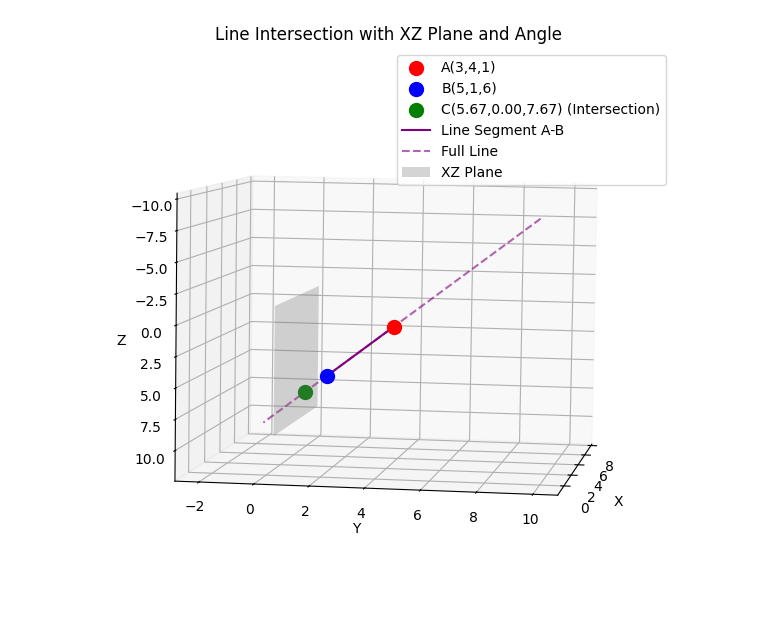
\includegraphics[width=0.8\columnwidth]{../figs/fig1.png}
\caption{}
\label{fig:1}
\end{figure}
\end{frame}
\begin{frame}{Plot by Python only}
\begin{figure}[H]
\centering
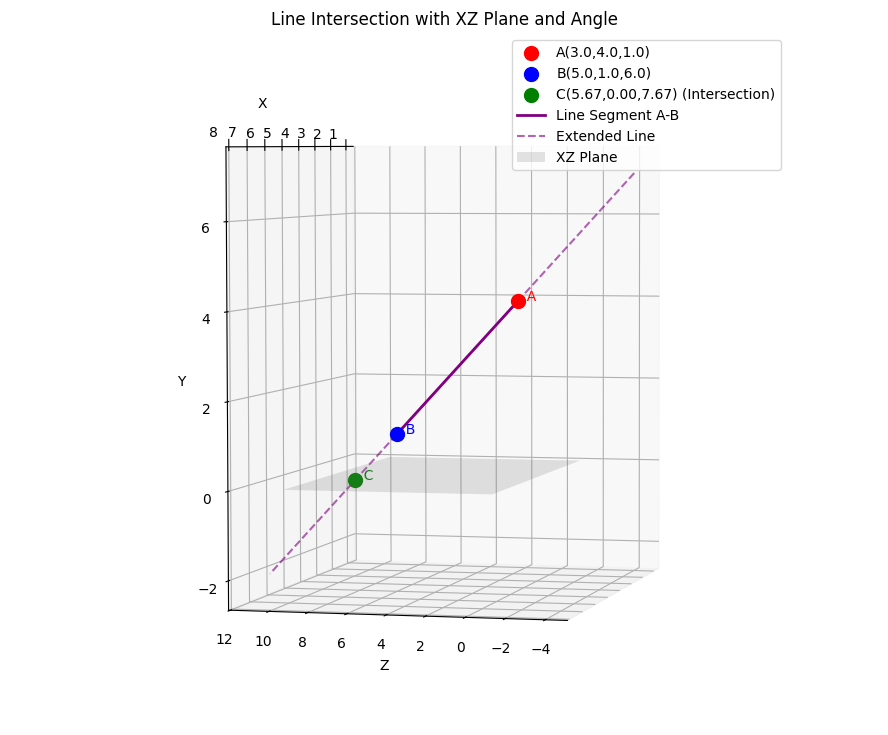
\includegraphics[width=0.8\columnwidth]{../figs/fig2.png}
\caption{}
\label{fig:2}
\end{figure}
\end{frame}
\end{document}
